%!TEX TS-program = xelatex

\documentclass {article}

\usepackage{xetexko}
\usepackage[a4paper]{geometry}
\usepackage[usenames,dvipsnames]{xcolor}
\usepackage{mathtools}
\usepackage{amsmath}
\usepackage{fontspec}
\usepackage{hyperref}
\usepackage{graphicx}
\usepackage{listings}
\usepackage{makeidx}
\usepackage{indentfirst}
\usepackage{tikz}
\usetikzlibrary{arrows,automata}


%\setmainfont {NanumMyeongjo}
\setmainfont {UnBatang}
\setmonofont[Scale=0.8]{DejaVu Sans Mono}

\lstdefinestyle{diff}{
  belowcaptionskip=1\baselineskip,
  breaklines=true,
  frame=L,
  xleftmargin=\parindent,
  showstringspaces=false,
  % Diffstart
  morecomment=[f][\color{gray}]{@@},
  % Diffincl
  morecomment=[f][\color{Green}]{+},
  % Diffrem
  morecomment=[f][\color{Red}]{-},
  basicstyle=\footnotesize\ttfamily,
}

\lstdefinestyle{customtxt}{
  belowcaptionskip=1\baselineskip,
  breaklines=true,
  frame=L,
  xleftmargin=\parindent,
  showstringspaces=false,
  basicstyle=\footnotesize\ttfamily,
}

\lstdefinestyle{customc}{
  belowcaptionskip=1\baselineskip,
  breaklines=true,
  frame=L,
  xleftmargin=\parindent,
  language=C,
  showstringspaces=false,
  basicstyle=\footnotesize\ttfamily,
  keywordstyle=\bfseries\color{green!40!black},
  commentstyle=\itshape\color{purple!40!black},
  identifierstyle=\color{blue},
  stringstyle=\color{orange},
}

\lstdefinestyle{customrs}{
  belowcaptionskip=1\baselineskip,
  breaklines=true,
  frame=L,
  xleftmargin=\parindent,
  showstringspaces=false,
  morekeywords={fn,let,mut,pub,use,impl,struct,unsafe,if,for},
  morecomment=[l]{//},
  morecomment=[n]{/*}{*/},
  basicstyle=\footnotesize\ttfamily,
  keywordstyle=\bfseries\color{green!40!black},
  commentstyle=\itshape\color{purple!40!black},
  identifierstyle=\color{blue},
  stringstyle=\color{orange},
}


\begin {document}

\title {Homework 1}
\input {../../reportauthor.tex}
\maketitle

Problem 1\newline
\indent $C_{space}$ represents space character and $C_{tab}$ represents tab character.
\begin{enumerate}
\item $c^*a(c+a)^*b(a+b+c)^*$
\item $((b+c)^*a(b+c)^*a(b+c)^*)^*$
\item $1(1+0)^*00$
\item $(C_{space} + C_{tab})^*$
\item \begin{align*}
  &whitespace \rightarrow (C_{space} + C_{tab}) \\
  &letter \rightarrow [a-zA-Z\_] \\
  &digit \rightarrow [0-9]
\end{align*}
  이라 하면,
  \begin{align*}
    (whitespace)^*//(whitespace|letter|digit)^*
  \end{align*}
\end{enumerate}

Problem 2\newline
\begin{enumerate}
\item
  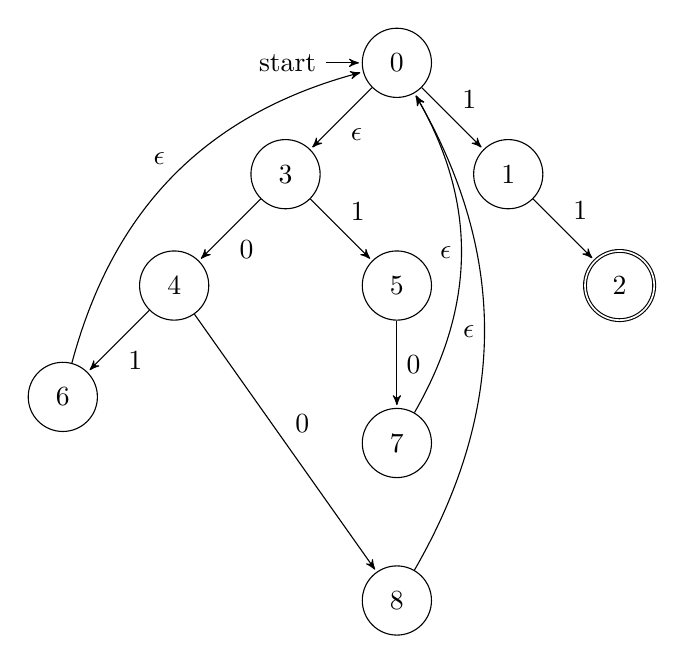
\begin{tikzpicture}[>=stealth',shorten >=1pt,auto,node distance=2cm]
%    \tikzstyle{every state}=[fill=white,draw=none,text=black]

    \node[initial,state]   (0)                    {0};
    \node[state]           (1) [below right of=0] {1};
    \node[state,accepting] (2) [below right of=1] {2};
    \node[state]           (3) [below left of=0]  {3};
    \node[state]           (4) [below left of=3]  {4};
    \node[state]           (5) [below right of=3] {5};
    \node[state]           (6) [below left of=4]  {6};
    \node[state]           (7) [below of=5]       {7};
    \node[state]           (8) [below of=7]       {8};

    \path [->]
    (0) edge node {1} (1)
    (1) edge node {1} (2)
    (0) edge node {$\epsilon$} (3)
    (3) edge node {0} (4)
    (3) edge node {1} (5)
    (4) edge node {1} (6)
    (4) edge node {0} (8)
    (5) edge node {0} (7)
    (6) edge [bend left] node {$\epsilon$} (0)
    (7) edge [bend right] node {$\epsilon$} (0)
    (8) edge [bend right] node {$\epsilon$} (0);
  \end{tikzpicture}
\item 모든 경우에서 $\epsilon$-closure 는 공집합이다.
\item
  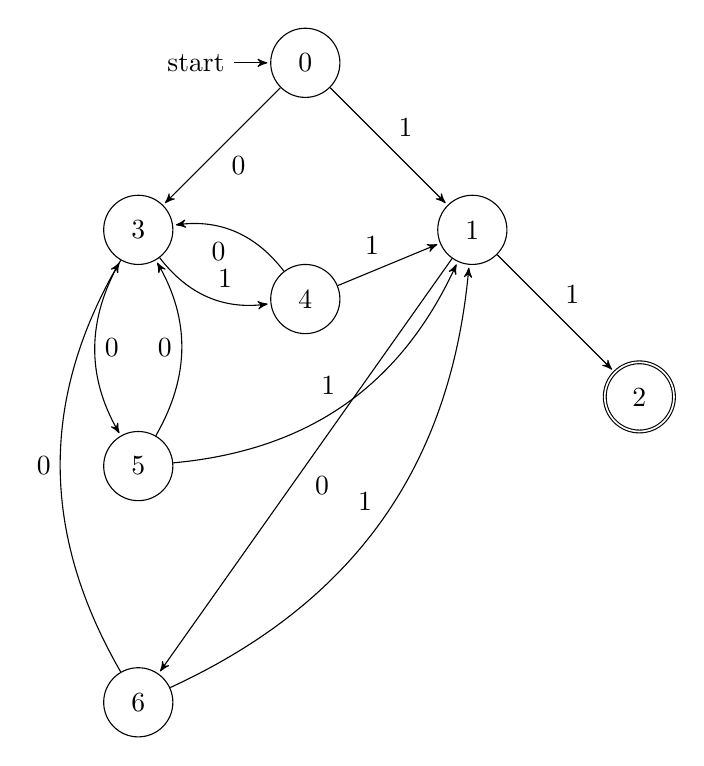
\begin{tikzpicture}[>=stealth',shorten >=1pt,auto,node distance=3cm]
    \node[initial,state]   (0)                    {0};
    \node[state]           (1) [below right of=0] {1};
    \node[state,accepting] (2) [below right of=1] {2};
    \node[state]           (3) [below left of=0]  {3};
    \node[state]           (4) [below of=0]       {4};
    \node[state]           (5) [below of=3] {5};
    \node[state]           (6) [below of=5]       {6};

    \path [->]
    (0) edge node {1} (1)
    (0) edge node {0} (3)
    (1) edge node {1} (2)
    (1) edge node {0} (6)
    (3) edge [bend right] node {1} (4)
    (3) edge [bend right] node {0} (5)
    (4) edge node {1} (1)
    (4) edge [bend right] node {0} (3)
    (5) edge [bend right] node {1} (1)
    (5) edge [bend right] node {0} (3)
    (6) edge [bend right] node {1} (1)
    (6) edge [bend left] node {0} (3);
  \end{tikzpicture}
\end{enumerate}
Problem 3\newline
\begin{enumerate}
\item
  \begin{align*}
    numbers &\rightarrow (1 + 2 + 3 + 4 + 5 + 6 + 7 + 8 + 9) \\
    integers &\rightarrow ((-) | (numbers)) | ((numbers) | (0))^* \\
    nil &\in L \\
    \text{if } l &\in L, \text{then } (integers) | l \in L \\
  \end{align*}
\item
  $Z$ 는 정수의 집합.
  \begin{align*}
    L &= fixF \\
    fixF &= ( F \cap Z ) \cup L \\
  \end{align*}
\end{enumerate}
\end {document}
